\section{諸群論的性質の定義}\label{group-theoretic-properties}

基本的な定義に関する辞書である。

\begin{defn}\label{0001}
  $G$ を副有限群とする。$\Class$ を有限群のクラスとする。$\Sigma \subset \Primes$ とする。
  \begin{enumerate}
    \item $G$ が center-free であるとは、$Z(G) = \{1\}$ であることをいう。
    \item $G$ が slim であるとは、任意の open subgroup $H \subset G$ に対して、$Z_G(H) = \{1\}$ であることをいう。
    \item $G$ が topologically finitely generated であるとは、$G$ が位相的有限生成であることをいう。
    \item $G$ が elastic であるとは、その topologically finitely generated な normal closed subgroup がすべて open あるいは自明であることをいう。
    \item $G$ が very elastic であるとは、$G$ が elastic であって、かつ $G$ が topologically finitely generated でないことをいう。
    \item $G$ が indecomposable であるとは、$G$ が非自明な積に分解できないことをいう。
    \item $G$ が strongly indecomposable であるとは、任意の open subgroup $H \subset G$ に対して、$H$ が indecomposable であることをいう。
    \item $G$ が finite であるとは、$G$ が有限群であることをいう。
    \item $G$ が infinite であるとは、$G$ が finite でないことをいう。
    \item $G$ が pro-$p$ であるとは、$G$ が $p$-群の inverse limit であることをいう。
    \item $G$ が almost pro-$p$ であるとは、$G$ が pro-$p$ な open subgroup をもつことをいう。
    \item $G$ が pro-$\Class$ であるとは、$G$ が $\Class$ に属する群の inverse limit であることをいう。
    \item $G$ が almost pro-$\Class$ であるとは、$G$ が pro-$\Class$ な open subgroup をもつことをいう。
    \item $G$ が自由副有限群 (free profinite group) であるとは、$G$ がある集合に対して副有限群として自由生成されていることをいう。副有限群であることが明らかな文脈では、単に自由群とよぶことがある。
    \item $G$ が free pro-$p$ group であるとは、$G$ がある集合に対して pro-$p$ group として自由生成されていることをいう。
    \item $G$ が free pro-$\Class$ group であるとは、$G$ がある集合に対して pro-$\Class$ group として自由生成されていることをいう。
    \item $G$ が cyclic であるとは、$G$ が $1$ 元生成されていることをいう。
    \item $G$ が profinite surface group であるとは、$G$ がある有限型 Riemann 面の基本群の副有限完備化と同型であることをいう。副有限群であることが明らかな文脈では、単に surface group とよぶことがある。
    \item $G$ が pro-$\ell$ surface group であるとは、$G$ がある有限型 Riemann 面の基本群の pro-$\ell$ 完備化と同型であることをいう。
    \item $G$ が GFGPC (geometric fundamental group of positive-characteristic curve) であるとは、$G$ がある正標数代数閉体上の代数曲線の基本群と同型であることをいう。
    \item $G$ が pro-$p$ GFGPC であるとは、$G$ がある標数 $p$ の代数閉体上の代数曲線の基本群の pro-$p$ 完備化と同型であることをいう。
    \item $G$ が NF-type であるとは、$G$ がある数体の絶対 Galois 群と同型であることをいう。(pro-$\Sigma$ NF-type などについても同様の用語法をおこなう。)
    \item $G$ が MLF-type であるとは、$G$ がある MLF の絶対 Galois 群と同型であることをいう。(pro-$\Sigma$ MLF-type, MLF$_p$-type, pro-$\Sigma$ MLF$_p$-type などについても同様の用語法をおこなう。)
    \item $G$ が PGF-type であるとは、$G$ がある PGF の絶対 Galois 群と同型であることをいう。(pro-$\Sigma$ PGF-type などについても同様の用語法をおこなう。)
    \item $G$ が PLF-type であるとは、$G$ がある PLF の絶対 Galois 群と同型であることをいう。(pro-$\Sigma$ PLF-type などについても同様の用語法をおこなう。)
    \item その他の体のクラスについても、同様の用語法をおこなう。
  \end{enumerate}
\end{defn}

以下の定義は、\cite{GeneralAnabGroupProp} によるものである。

\begin{defn}\label{0003}
  $G$ を位相群とする。$n$ を自然数とする。
  \begin{enumerate}
    \item $H \subset G$ を部分群とする。$n \in \Nzero$ とする。このとき、$H$ が $G$ において $n$-subnormal であるとは、$H_0 = G$, $H_n = H$ であるような部分群の列 $H_0 \supset H_1 \supset \cdots \supset H_n$ が存在して、任意の $i = 1, \ldots, n$ について、$H_i$ が $H_{i - 1}$ において normal であるようにできることをいう。$H$ が $G$ において subnormal であるとは、ある $n \in \Nzero$ について、$H$ が $G$ において $n$-subnormal であることをいう。
    \item $H \subset G$ を部分群とする。$H$ が $G$ において normally decomposable であるとは、$H$ が $G$ の非自明な正規部分群 $H_1$, $H_2$ によって $H = H_1 \times H_2$ と分解できることをいう。$H$ が $G$ において normally indecomposable であるとは、$H$ が $G$ において normally decomposable でないことをいう。
    \item $G$ が internally indecomposable であるとは、任意の $G$ の非自明な正規部分群が center-free であり、かつ normally indecomposable であることをいう。$G$ が副有限群であるとき、$G$ が strongly internally indecomposable であるとは、任意の open subgroup $H \subset G$ に対して、$H$ が internally indecomposable であることをいう。
    \item $G$ が $n$-sn-internally indecomposable であるとは、任意の $G$ の $(n - 1)$-subnormal な部分群が internally indecomposable であることをいう。
    \item $G$ が副有限群であるとき、$G$ が strongly $n$-sn-internally indecomposable であるとは、任意の open subgroup $H \subset G$ に対して、$H$ が $n$-sn-internally indecomposable であることをいう。
    \item $G$ が sn-internally indecomposable であるとは、ある $n \in \N$ について、$G$ が $n$-sn-internally indecomposable であることをいう。
    \item $G$ が副有限群であるとき、$G$ が strongly sn-internally indecomposable であるとは、任意の open subgroup $H \subset G$ に対して、$H$ が sn-internally indecomposable であることをいう。
    \item $G$ が副有限群であるとき、$G$ が $n$-sn-quasielastic であるとは、任意の $G$ の topologically finitely generated な $n$-subnormal closed subgroup が自明あるいは open であることをいう。
    \item $G$ が副有限群であるとき、$G$ が $n$-sn-elastic であるとは、任意の $G$ の開部分群の topologically finitely generated な $n$-subnormal closed subgroup が自明あるいは open であることをいう。
    \item $G$ が quasi-elastic であるとは、$G$ が $1$-sn-quasielastic であることをいう。
    \item $G$ が sn-quasielastic であるとは、ある $n \in \N$ について、$G$ が $n$-sn-quasielastic であることをいう。
    \item $G$ が sn-elastic であるとは、ある $n \in \N$ について、$G$ が $n$-sn-elastic であることをいう。
    \item $G$ が very quasielastic (resp., very $n$-sn-quasielastic, very $n$-sn-elastic, very sn-quasielastic, very sn-elastic) であるとは、$G$ が quasi-elastic (resp., $n$-sn-quasielastic, $n$-sn-elastic, sn-quasielastic, sn-elastic) であって、かつ $G$ が topologically finitely generated でないことをいう。
  \end{enumerate}
\end{defn}

\begin{defn}\label{0004}
  副有限群 $G$ について、全射 $G \to Q$ が almost pro-$\Class$ maximal quotient であるとは、ある $G$ の normal open subgroup $H$ が存在して、$G \to Q$ の kernel が $H \to H^p$ の kernel と一致することをいう。
\end{defn}

\section{諸群論的性質についての純群論的事実}

\begin{lem}\label{0002}
  $G$ を副有限群とする。このとき、$G$ が topologically finitely generated かつ elastic であるならば、$G$ は indecomposable であるか、あるいは有限群である。
\end{lem}
\begin{proof}
  $G = G_1 \times G_2$ として非自明な分解があるとする。このとき、$G_1$, $G_2$ はいずれも topologically finitely generated な normal closed subgroup であるため、指数有限である。したがって、$G$ は有限群である。
\end{proof}

\begin{defn}\label{0007}
  $G$ を位相群とする。$G$ が internally infinite であるとは、$G$ の非自明な normal closed subgroup がすべて infinite であることをいう。
\end{defn}

\begin{lem}\label{0006}
  $G$ を副有限群とする。このとき、$G$ が slim であるならば、$G$ は internally infinite である。
\end{lem}
\begin{proof}
  conjugation による準同型 $G \to \Aut(H)$ をみるとき、この kernel を $U$ とおくと、$Z_G(U) \supset H \neq 1$ であり、これは slimness に矛盾する。 
\end{proof}

\begin{lem}\label{0009}
  $G$ を副有限群とする。$G$ が internally infinite であるとする。$N$ を $G$ の normal closed subgroup であり、また $H$ を $G$ の open subgroup とする。このとき、$N \cap H = 1$ ならば、$N = 1$ である。
\end{lem}
\begin{proof}
  $N$ の有限性より、補題は形式的である。
\end{proof}

\begin{lem}\label{000H}
  $G$ を副有限群とする。このとき、$G$ が topologically finitely generated であれば、その開部分群もまた topologically finitely generated である。
\end{lem}
\begin{proof}
  自由群に関する議論に帰着される。
\end{proof}

\begin{lem}\label{000I}
  $G$ を副有限群とする。このとき、$G$ が very elastic であることと、$G$ が nontrivial な topologically finitely generated normal closed subgroup をもたないことは同値である。
\end{lem}
\begin{proof}
  Lemma \ref{000H} をもちいれば、簡単である。
\end{proof}

以下の内容は、\cite{IntIndecomp} によるものである。

\begin{lem}[internal indecomposability についての簡単な基準]\label{0005}
  $G$ を副有限群とする。このとき、$G$ が internally indecomposable であることと、任意の nontrivial normal closed subgroup $H$ について $Z_G(H) = \{1\}$ であることは同値である。
\end{lem}
\begin{proof}
  両方向を確認する。
  \begin{itemize}
    \item $G$ が internally indecomposable であるとする。このとき、nontrivial な normal closed subgroup $H$ について、以下が成り立つ。
    \begin{itemize}
      \item $Z_G(H) \cap H = 1$ ($H$ の center-free 性).
      \item $H$ と $Z_G(H)$ はともに $G$ で normal である。
      \item $H$ と $Z_G(H)$ は可換する。
    \end{itemize}
    よって、$H \times Z_G(H) \subset G$ は $G$ で normal な部分群による分解となるが、これは $H = 1$ あるいは $Z_G(H) = 1$ を意味する。
    \item 任意の nontrivial normal closed subgroup $H$ について $Z_G(H) = 1$ であることを仮定する。このとき、nontrivial な normal closed subgroup $H$ について、$Z(H) \subset Z_G(H) = 1$ である (center-free)。また、$H = H_1 \times H_2$ なる非自明な $G$ の正規部分群による分解があれば、$Z_{G}(H_1)$ は $H_2$ を含む。
  \end{itemize}
  これは補題の証明である。
\end{proof}

\begin{rem}\label{000F}
  以下の類似を確認したい:
  \begin{itemize}
    \item $G$ が slim であるとは、任意の open subgroup $H$ に対して、$Z_G(H) = \{1\}$ であることをいう。
    \item $G$ が internally indecomposable であるとは、任意の nontrivial normal closed subgroup $H$ に対して、$Z_G(H) = 1$ であることをいう。
  \end{itemize}
  この意味で、``internally indecomposable'' とは、ある種の正当な ``slim'' の強化であるといえる。
\end{rem}

\begin{lem}[internal indecomposability について、開部分群からの ascend]\label{0008}
  $G$ を副有限群とする。$G$ を internally infinite であると仮定する。このとき、$G$ の開部分群 $H$ が internally indecomposable であるならば、$G$ もまた internally indecomposable である。同様に、$H$ が strongly internally indecomposable であるならば、$G$ もまた strongly internally indecomposable である。
\end{lem}
\begin{proof}
  \begin{itemize}
    \item strongly internally indecomposable の場合は、前半の部分から形式的に従う。
  \end{itemize}
  internally indecomposable の場合は、(Lemma \ref{0009} をもちいて、)Lemma \ref{0005} からただちに従うことが確認できる。(すなわち、$N$ を $G$ の nontrivial な normal closed subgroup とする。このとき、$N \cap H \neq 1$ であるため、$Z_H(N \cap H) = 1$ である。したがって、$Z_G(N) = 1$ が導かれる。)
\end{proof}

\begin{lem}[internal indecomposability について、surjective system に関する極限への ascend]\label{000A}
  $G$ を副有限群とする。$\{N_i\}_{i \in I}$ を $G$ の normal closed subgroup による separated な directed system とする (順序は狭方を大とする)。このとき、$G/N_i$ ($i \in I$) がすべて internally indecomposable であるならば、$G$ もまた internally indecomposable である。また、$G/N_i$ ($i \in I$) がすべて strongly internally indecomposable であるならば、$G$ もまた strongly internally indecomposable である。
\end{lem}
\begin{proof}
  \begin{itemize}
    \item strongly internally indecomposable の場合は、前半の部分から形式的に従う。
  \end{itemize}
  internally indecomposable の場合について: $N$ を $G$ の nontrivial な normal closed subgroup とする。$C$ を $N$ の centralizer とする。このとき、$N$ も $C$ も像が活きている添字にうつれば、その添字で矛盾が生じる。したがって、等式 $C = 1$ がみちびかれる。
\end{proof}

\begin{lem}[自己同型に関するトリック]\label{000B}
  $G$ を副有限群とする。$G$ が internally indecomposable であるとする。$H$ を $G$ の nontrivial な normal closed subgroup とする。このとき、$\alpha \in \Aut(G)$ であって、$\alpha|_H = \id_H$ であるものは、恒等射
  に限られる。
\end{lem}
\begin{proof}
  $\alpha(g) \cdot g^{-1}$ を $\beta(g)$ とおいたとき、$\beta(g) \in Z_G(H)$ となることが確認できる。したがって、$\beta(g) = 1$ であるため、$\alpha(g) = g$ である。
\end{proof}

\begin{lem}[自己同型に関するトリック - variant 1]\label{000C}
  $G$ を副有限群とする。$H$ を $G$ の normal subgroup とする。$\alpha \in \Aut(G)$ について、これが $\alpha|_H = \id_H$ を充たすとする。このとき、$g \in G$ について、$\alpha(g) \cdot g^{-1} \in Z_G(H)$ である。
\end{lem}
\begin{proof}
  Lemma \ref{000B} とおなじ議論である。
\end{proof}

\begin{lem}[自己同型に関するトリック - variant 2]\label{000D}
  $G$ を slim な副有限群とする。このとき、$\alpha \in \Aut(G)$ であって、開部分群 $U$ 上で identity であるものは identity に限られる。同様に、$U$ 上で inner automorphism であるものは、($U$ の元による) inner automorphism に限られる。
\end{lem}
\begin{proof}
  Lemma \ref{000C} の直接の帰結である。
\end{proof}

\begin{lem}[internal indecomposability について、extension への ascend]\label{000E}
  以下に、副有限群の可換図式をとる。
  \begin{center}
    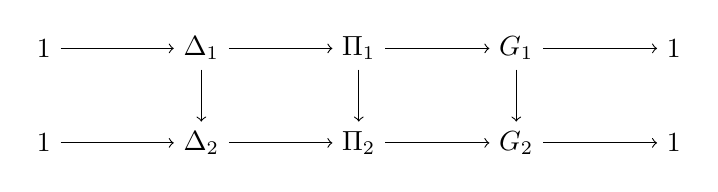
\begin{tikzpicture}
      \node (A1) at (0, 0) {$1$};
      \node (B1) at (2, 0) {$\Delta_1$};
      \node (C1) at (4, 0) {$\Pi_1$};
      \node (D1) at (6, 0) {$G_1$};
      \node (E1) at (8, 0) {$1$};
      \node (A2) at (0, -1.2) {$1$};
      \node (B2) at (2, -1.2) {$\Delta_2$};
      \node (C2) at (4, -1.2) {$\Pi_2$};
      \node (D2) at (6, -1.2) {$G_2$};
      \node (E2) at (8, -1.2) {$1$};
      \draw[->] (A1) to node[above] {} (B1);
      \draw[->] (B1) to node[above] {} (C1);
      \draw[->] (C1) to node[above] {} (D1);
      \draw[->] (D1) to node[above] {} (E1);
      \draw[->] (A2) to node[above] {} (B2);
      \draw[->] (B2) to node[above] {} (C2);
      \draw[->] (C2) to node[above] {} (D2);
      \draw[->] (D2) to node[above] {} (E2);
      \draw[->] (B1) to node[right] {} (B2);
      \draw[->] (C1) to node[right] {} (C2);
      \draw[->] (D1) to node[right] {} (D2);
    \end{tikzpicture}
  \end{center}
\end{lem}
ここで、垂直の射がすべて open injection であったとする。またそれぞれの行によってつくられる外表現を $\rho_1: G_1 \to \Out(\Delta_1)$, $\rho_2: G_2 \to \Out(\Delta_2)$ とする。このとき、$\Ker{\rho_1} \subset \Ker{\rho_2}$ である。とくに、$\rho_2$ が単射ならば、$\rho_1$ もまた単射である。
\begin{proof}
  Lemma \ref{000D} をもちいれば、簡単である。
\end{proof}

\begin{prop}\label{000G}
  \[
    1 \to \Delta \to \Pi \to G \to 1
  \]
  を副有限群の完全列とする。また、この完全列に付随する外表現を $\rho: G \to \Out(\Delta)$ とする。このとき、以下が成立する。
  \begin{enumerate}
  \item $\Delta$, $G$ いずれも internally indecomposable であり、かつ $\rho$ が単射であるならば、$\Pi$ もまた internally indecomposable である。同様のことが strongly internally indecomposable についても成り立つ。
  \item $\Delta$ が internally indecomposable であって、$G$ が abelian であるとする。このとき、$\rho$ の単射か、あるいは $\Pi$ の center-free があれば、$\Pi$ は internally indecomposable である。同様のことが strongly internally indecomposable についても ($\rho$ の単射あるいは $\Pi$ の slimness により) 従う。
  \end{enumerate}
\end{prop}
\begin{proof}
  open subgroup に下がっても (f\'{e}t に上がっても)、外表現の単射が成り立つというのが Lemma \ref{000E} である。このことをみれば、strongly ... 側は形式的である。
  \begin{enumerate}
    \item $N$ と $C$ が $\Pi$ の normal closed subgroup であって、これらが可換すると仮定する。すれば、$\rho$ の単射と Lemma \ref{000B} の trick により、いずれかが $\Delta$ において非自明に交わり、もう一方が $G$ において活きているという状況を封じる。しかし、それぞれの internal indecomposability は $\Delta$ においてともに活きること、$G$ においてともに活きることを封じる。これはいずれかの自明性をみちびく。
    \item $\rho$ が単射なら、$\Pi$ が center-free であることは簡単にわかる。ここで、$H$ が非自明な $\Pi$ の normal closed subgroup であれば $H \cap \Delta \neq 1$ であることを確認する: $1 \neq h \in H$ について、$[g, h] \neq 1$ なる $g \in \Pi$ が存在する (center-free 性より)。$[g, h] \in H \cap \Delta$ であるので、これは claim をみちびく。このことを $N$ と $C$ の議論に適用すれば $\Delta$ の internal indecomposability から状況は従う。
  \end{enumerate}
  これは命題の証明である。
\end{proof}

\section{体の絶対 Galois 群に対する slimness}

\section{体の絶対 Galois 群に対する elasticity}

\section{体の絶対 Galois 群に対する indecomposability}

\section{曲線の基本群に対する slimness}

\section{曲線の基本群に対する elasticity}

\section{曲線の基本群に対する indecomposability}

\section{$\Out(F)$, $F$: 自由群 of rank $ \geq 2$, に対する strongly indecomposability}

以下は、

\section{$\GT_\ell$ に対するindecomposability}